\chapter{Far Out Memory Hierarchies}\label{ch:farout}

\section{Persistence and Distibution}


\unedit{
    The first key characteristic of \NVM is
    low latency: only $1.5$--$8\times$ the
    latency of DRAM in most cases~\cite{ucsd_bnvm}. Thus the cost of a system call to
    access \NVM
    %($0.5$--\SI{1}{\micro\second})
    dominates the
    latency of the access itself. The second key characteristic is that the processor can directly
    access persistent storage using load and store instructions.
    Direct, low latency access to \NVM means that explicit
    serialization is a poor fit---it adds complexity, as programmers must maintain different
    data formats and the transformations between them, and the overhead is intolerable due to \NVM's
    low latency. Hence, we should design the semantics of the programming model around
    \emph{in-memory} persistent data structures, giving programs direct access to them without
    explicit persistence calls or serialization methods.
}


\section{Memory Capacity}

\section{Increasing Hardware Complexity and Performance}

\unedit{
    \begin{figure}
        \centering
        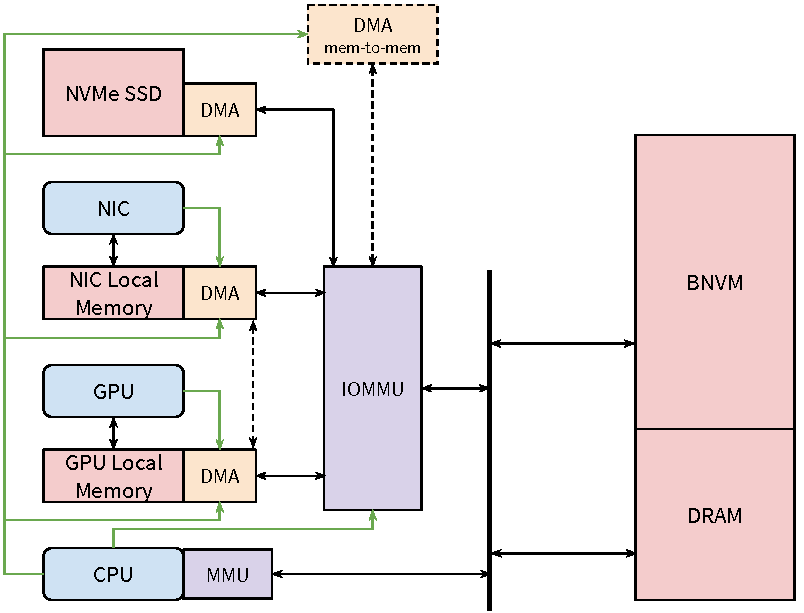
\includegraphics[width=\linewidth]{fig/sys_arch}
        \caption{Our expected system architecture. Solid black lines indicate data paths, green lines
            indicate administration paths. Dashed lines and boxes indicate potential future data paths and hardware
            that may become ubiquitous with these new hardware trends.}
        \label{fig:sys_arch}
    \end{figure}


    A second trend is a consequence of improved fabrication techniques and shrinking feature
    sizes---hardware controllers are increasing in complexity, offering more autonomy from the CPU,
    off-CPU processing capabilities, and better parallelism. Hardware interfaces reflect the controller
    complexity expected of devices; for example, AHCI controllers improved request queuing over ATA, and DMA
    allows hardware to copy data directly to and from memory independent from the CPU. NVMe
    expands the responsibility of controllers again, adding deeper and parallel command queues, requiring
    devices to multiplex requests themselves and allowing them to exploit the parallelism of access
    available in SSDs. We expect these trends to continue, resulting in more programmable hardware
    devices that are able to act on shared, global memory with more autonomy.

    These changes are coupled with a shift in focus for how data moves throughout the system.
    Traditionally, data is considered to move into main memory for computation by the CPU, followed by
    storage to persistent memory (through a disk or SSD controller) or moved out onto the network
    (through a network controller). Figure~\ref{fig:sys_arch} shows a different model, where data moves
    through the system more fluidly. With more complex controllers and off-CPU processing, we expect
    non-traditional data paths to become more common. Say, for example, a packet arrives at the NIC
    containing compressed data for GPU processing. A traditional system would move the compressed data
    into main memory, decompress it using the CPU, and move it into GPU memory for processing. Instead,
    we could see a dedicated compression chip in the NIC whose job it is to decompress incoming data.
    That data could then be moved directly between the NIC's buffers and the GPU memory (the dashed
    line), without involving the CPU and main memory at all. This both reduces copies and frees these
    resources for other uses.
}


\subsection{Interconnect Technologies}

\section{Why Now?}
